\chapter[SCP-001 孩子们]{
	SCP-001 djkaktus - The Children \\
	SCP-001 孩子们
}

\label{chap:SCP-001.the.children}

\newcommand{\vdotsc}[1]{\cl{\multido{}{#1}{. \\}}}

\begin{scpboxbbwmc}
\GG{\wred{\bb{警告:以下文件被分类为}}}

\Hg{\wred{\bb{5级}}}

\GG{\wred{\bb{此分类由监督者议会授权}}}

\Gg{\bb{任何未经5级授权试图访问该文件的行为将被记录,并且查阅者将被处决。}}
\end{scpboxbbwmc}

\hr

\vdotsc{7}

\begin{scpboxc}
输入五级基本安保证书
\end{scpboxc}

\vdotsc{7}

\begin{scpboxc}
Command:\textbackslash users\textbackslash O513>\_ 6110298-父罪与子罪-3561840
\end{scpboxc}

\vdotsc{7}

\begin{scpboxc}
允许访问,初级模因抹杀剂解除,晚上好,O5-13。
\end{scpboxc}

\vdotsc{7}

\begin{scpboxc}
警告:此文档部分内容已被锁定。
\end{scpboxc}

\begin{scpboxc}
解锁需要额外的5级权限。
\end{scpboxc}

\vdotsc{7}

\hrule

\begin{figure}[H]
	\centering
	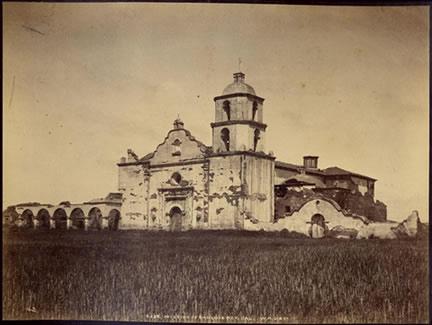
\includegraphics[width=0.5\linewidth]{images/SCP.001.the.children.jpg}
	\caption{位于墨西哥圣马可的San Marcos de la Vida Eterna教堂,\\ 照片上的日期为07/27/1903}
\end{figure}

\bb{项目指定编号:}Item-001

\bb{收容等级:}Keter-Thaumiel

\bb{收容状态:}激活-稳定

\bb{收容措施:} 物体-001(Item-001)现在正被收容于墨西哥的圣马可,收容地点位于San Marcos de la Vida Eterna教堂的旧址地下。原始收容措施已经证明可以有效收容物体-001。收容区域现在被指定为一个高安保级别的军队废物处理厂,墨西哥法律则禁止所有平民接近该站点10km范围内。围绕物体-001的收容区域将有自动化闭路监控无人机进行巡逻,并且这些无人机被设计为一旦见人将格杀勿论。

\bb{O5备忘录001-Alpha:}\ii{对于有关SCP-001,也就是前物体-001,的所有信息收容将成为最高优先事项。我已经授权将资料库之中相关资料清除,并在原地址上创建数个错误项目。如果真的有人能追查到那个地址,那些伪装项目也足够让他们感到失望了。我现在抽出了好几个EX的SCP项目放置在那个地址上,直到我们找到更好的伪装项目为止。}

\ii{删除你找到的任何信息,堵住任何可能的漏洞,将这些信息掩埋在你觉得足够多的模因抹杀剂之下。要做到这一点,你需要做比完全删除资料还要多的多的工作。-O5-2}

\bb{项目描述:}物体-001是对9名人类组成的群体的指称,这些人年龄在4-11岁不等.他们因为001项目:“神之双子”(Twins of God)(见项目提案001以获得更多信息)而取得了异常性质。因为对物体-001进行了不当使用,导致了一名高级人员的死亡,这也使得对其进行处决变得必要。作为这一事件的结果,物体-001现在按照现有收容措施进行了收容。所有9名物体-001的个体都在功能上已经进入了脑死亡状态,但却仍然表现出生命体征,而不论对其的收容措施情况如何。

物体-001的个体都放射出大量的伽马射线,放射量通常都在███GJ以上,并且以一种独特的形式进行变换。当每个个体单独收容时,这种放射模式似乎是随机的,但如果将这些个体进行集合收容时,这些放射模式似乎会出现某种确定的特征。因此,每一个个体之间收容间隔大约应保持在████。另外值得注意的是,物体-001的个体是具有辐射发光性的。在这些个体进入激活状态时,对它们进行视频监控是不可能的,因为在此状态下的个体出现在屏幕中时将导致录影脚本发生损坏。

当一个物体-001个体与其他个体之间相隔小于20m时,它将表现出对物体、人类个体或是某块区域的远距离毁灭能力。对于此性质将会稍后在此文档之中进行详细描述。

根据监督者议会的命令,物体-001被分类为一个Thaumiel\footnote{"Humphrey, W., Lemke, R., Christian, K., Roesler, J., \& Kaiser, N,(1920),《收容分级提案:Thaumiel》,基金会研究出版社,2(7)。"}-Keter实体。

\vs\hrule

\begin{scpboxbbwm}
\bb{警告:}有关物体-001的更多信息已经锁定,并且已经被分类为5级。模因抹杀剂已经插入其中保证有关于物体-001的信息不会出现外泄。非监督者议会成员,并且不具备5级模因抵抗条件的人员将会受到模因抹杀剂影响而被处决。\bb{\ii{你已受到警告,并且这是最终警告。}}
\end{scpboxbbwm}

\cl{\bb{项目提案001: 锁定}}

\cl{\tred{+ 输入授权密码}}

\cl{\tred{1485992-13人乘死者船-4910581}}

\begin{scpboxc}
{[模因抹杀剂无效化]}
\end{scpboxc}

\begin{scpboxbbwm}
\GG{\bb{\tred{项目提案:“神之双子”}}}

\Gg{研究团队:Omega-5}

\g{\bb{项目日期:02/13/1922}}

\Gg{\bb{目的阐述:}}

\ii{此项目旨在创造出一个异常实体,该实体能在基金会中心高层必要的掌控之下,对基金会及全球安全造成威胁的敌意异常个体加以远距离摧毁。}

\bb{研究团队主任:} Dr. ███ █████, Ph.D. (O5-1)

\bb{副主任:} ████ ██████ (O5-2),████ ████ (O5-3)

\Gg{\bb{项目需求:}}

\begin{itemize}
	\item 取得并且使用物体-███:“亚原子加速系统”。
	\item 取得并且使用物体-███:“Harken之门”。
	\item 取得并且使用物体-███:“多重注射器”。
	\item 能够制造必要收容措施和研究设施的材料。
	\item 不少于50名成年人类个体(D级)作为测试目的之用。
\end{itemize}
	
\Gg{\bb{项目细节:}}

通过分析最近从物体-███和物体-███实验之中取得的信息,一个之前不可能出现的机会摆在了基金会面前:一种能力,能够穿越远距离改变物体量子组成,从而导致该物体从功能上不复存在\footnote{Maxwell, T., \& Gouram, A.(1927),《远距离上的量子性质》,基金会研究出版社,05(02),213-230页。}的能力。到目前为止,通过使用物体-███来改变人体性质从而对这一效应加以更大的操控,我们认为这一点是可以做到的。为了达到我们的最终目的,物体-███、物体-███和物体-███已经从基金会记录之中抹消了,并且它们将会单独收容在这个项目最初的研究设施之中。

在美国核试验设施的幌子之下,我们将在墨西哥北部建立一个站点,远离人群,这也是出于对这一理论进行安全测试的考虑。为了将这些实验对自然性质可能造成的潜在影响降到最小,我们将对这一项目进行最高的防护措施,对灾难性收容失效事件也建立了数个意外保险措施。这些保险措施将会在下面列出。

如果这一项目最终成功,这些实验创造的实体,暂时指定为物体-001的控制权,将交由基金会管理者掌控来对抗我们指定为GOI-003“地狱王国”(Kingdom of Abbadon)的异常敌对组织,一系列心灵抹杀剂将植入这些实体之中,对于这些抹杀剂的取得也只对管理者单独开放,这是作为确保这些个体不会落入敌对组织控制之中的保险措施。

\end{scpboxbbwm}

\begin{scpboxc}
{[模因抹杀剂无效化]}
\end{scpboxc}

\begin{scpboxbbwm}

\GG{\bb{意外保险收容措施:}}

\bb{Alpha:} 当出现灾难性收容失效事件时,植入这些实体之中的心理抹杀剂将启动,将其处决。每一种抹杀剂都被赋予不同的优先级并且应按顺序使用,以下是优先性列表:

\begin{itemize}
	\item Berkeley剂:降低身体活动能力。
	\item Anastasia剂:降低异常性质[正在开发中]。
	\item Nezbit剂:降低心理能力。
	\item Orion剂:对高级神经系统的全面化学性溶解。
\end{itemize}

\bb{Beta:} 在Alpha保险措施失效的情况下,安保人员应前去处决物体-001。将这些个体捕获的可能性不大,也不推荐这么做。建议相关人员与物体-001个体之间保持安全作业距离,并且穿着必要的基金会开发的反辐射防护装甲。同时推荐进行远距离弹道射击,因为这一行动将不会那么快吸引物体-001个体的注意。

\bb{Delta:}在Beta保险措施失效的情况下,基金会控制的长距离弹道武器将启动并且直接作用于物体-001个体上。我们将在研究设施外建立一个10km的边界,不少于10架重装轰击加农炮部署于这一边界上。在Delta措施启动时,它们将用于处决物体-001。

\bb{Epsilon:}在Delta保险措施失效的情况下,站点自身装载的自爆装置将启动,基金会管理者将全程监督Epsilon措施的实施情况。

\Gg{\bb{项目批准:}}

\begin{figure}[H]
	\captionsetup{singlelinecheck=false}
	
\includegraphics{images/SCP.001.the.children.2.png}
	\caption*{\ii{基金会管理者 R. D. Fritzwilliams}}
\end{figure}

\begin{figure}[H]
	\captionsetup{singlelinecheck=false}
	
\includegraphics{images/SCP.001.the.children.3.png}
	\caption*{\ii{项目主任O5-1}}
\end{figure}

\end{scpboxbbwm}

\cl{\bb{项目报告001-Delta: 锁定}}

\cl{\tred{+ 输入授权密码}}

\cl{\tred{- 7483529-九分钟后午夜-1889475}}

\begin{scpboxc}
{[模因抹杀剂无效化]}
\end{scpboxc}

\begin{scpboxbbwm}

\GG{\bb{\tred{项目“神之双子”进程报告}}}

\Gg{研究团队:Omega-5}

\g{\bb{项目日期:04/18/1924}}

\bb{进展细节:}

对于新物体-001个体的收容立刻就出现了问题,因为在约35\%活跃项目人员之中产生的[从记录之中删除]和急性放射病,我们出现了█人伤亡。对于收容措施的调整变得很有必要,以及这个现在我们指定为站点-001的站点内部结构也进行了强化。人员的住所已经后撤到了一处里主要研究设施有5km远的地方。

在苏丹,一次由地狱王国主导的对基金会设施袭击再次加剧了对远距离防卫系统的紧急需求,也同时加快了激活物体-001的时间表。在基金会管理者的命令下,我们得到了额外的物资来发展更为高效的实验设施。

另一件核心要件则是如何将异常性质收容在一个人类个体之中。在所有100\%的实验个体之中,尽管异常性质都只出现了一些小事故就能收容在他们体内,但所有的实验个体都会立刻瘫痪并且出现严重的脑溢血。而异常性质发挥效用的唯一证据则是站点结构或人员的随机突发毁灭,理论认为这一现象是因实验个体心理控制力恶化,无从控制这些异常性质而导致的。在所有100\%这些情况下,我们都启动了心理抹杀剂来将这些前物体-001个体处决。

站点外人员主导的另一项实验给了我们灵感,或许将这种异常性质平均分散到数个人类个体体内是可能的\footnote{Enjilian, M., \& Johnson, R.(1923)《数个Keter项目的异常性质》,基金会研究出版社,1(11)。},如此一来异常性质对人类个体心灵造成的压力问题将得以解决\footnote{Everly, K., \& Everly, J.(1922)《被消灭的Keter实体的大脑结构:对超自然个体认知结构的进一步分析》(第三版,第一章,自费出版,145-178页)芝加哥,IL:基金会科学出版社。}。

在一次使001号站点运转能力降低的测试,以及在基金会管理者命令下将D级人员转出站点到其他课题的行动之后,我们不得不讨论项目是否能继续进行这一问题。在与17号站点的主任进行咨询之后,一队武装特工进驻了墨西哥圣马可的San Marcos de la Vida Eterna教堂,并且他们还找来了一群年轻人进行测试。我们对圣马可城全体市民都进行了A级记忆消除,而这些人则之后被转送到了09号站点以备下一步之用。圣马可城本身则成为了新的001测试站点,23名最健康的个体被挑选出来进行实验,而剩余个体则全数处决。

\end{scpboxbbwm}

\begin{scpboxc}
{[模因抹杀剂无效化]}
\end{scpboxc}

\begin{scpboxbbwm}

\Gg{现状:}

现在这个项目准备进入下一阶段,下一阶段的实验将会在新的001测试体上进行,这一实验还在等待来自中央控制层的命令。以下这封信是申请将项目推进到下一阶段的,内容如下:

\begin{scpbox}

04/03/1924 \\
致:基金会管理者 \\
自:Omega-5团队负责人

管理者Fritzwilliams:

正因为从您办公室之中发出的每一条缩减预算和削减补给的命令,我们的项目随着每一条这种命令的发出而越来越难以保持进度。在中央控制层还没有主动与我们进行联系的情况下,我们只能认为对我们的指示是不变的。

一份为帮助我们项目尽快获得结果而寻求物资帮助的申请很快也会到达您那里,我们希望您能看到形势的变化,并且给我们的一个良好的答复。如能及时回信,不胜感谢。

███ █████ \\
项目负责人

\end{scpbox}

04/15/1924 \\
致:Omega-5团队负责人 \\
自:基金会管理者

█████:

我们给你下达的指令依然没有改变。如果你们的项目能够成功,那么我们就大可高枕无忧了。但很不幸的是,严酷的事实时刻提醒着我们,我们身陷一场战争之中,而物资又是如此贫乏。为了保证我们事业的隐秘性,我们再没有面对过比这状况更严峻的时期了,更不要谈继续你们的研究。但我仍会尽我一切努力帮助你们,不为别的,只因为你们的研究能从地狱王国手中保护我们。

我已经接到了你们的申请,尽管从道德上我没有任何理由去批准它,但我作为基金会领导者还是强迫自己批准了它。市民随便你们挑,但只允许挑成年人,也不要肆意践踏无辜者的生命。上帝知道,为了我们的目的已经有足够多的无辜者鲜血洒下了,我不希望再看到更多。

管理者Fritzwilliams \\
基金会中央管理层

\end{scpboxbbwm}

\cl{\bb{文档:GOI-3“地狱王国”: 锁定}}

\cl{\tred{+ 输入授权密码}}

\cl{\tred{- 4561273-影覆沙丘-0948390}}

\begin{scpboxbbwm}

\GG{\bb{\tred{同行组织文档003}}}

\Gg{\bb{指称:地狱王国(Kingdom of Abbadon)}}

\bb{威胁等级:}非常高 \\
\bb{活跃等级:}非常高 \\
\bb{优先度:}5级

\bb{综述:}GOI-003“地狱王国”是对一群异常敌对人性个体的指称,他们现在位于撒哈拉沙漠的某处,该处根据其手稿之中的描述被称为“吾等神王Abbadon之城”。这些人形个体从很多方面都与人类相似,但他们所有成员都至少是I级现实扭曲个体。\footnote{Benson, R.(1921)《现实扭曲个体分级》,基金会研究出版社,3(7),10-58页。},同时高级个体已经达到了III级或者IV级的现实扭曲分类。由于他们本身异常性质之强烈,对它们的捕获和收容是不可能的,并且任何这方面的尝试都十分危险。

\bb{最初发现:}GOI-003最初是由法国军队人员于1912年,对一起利比亚北部村落的袭击行为调查之中发现的。军队的护卫队遭到了袭击,80\%的人员死亡。幸存者称他们被不多于6个人的“巫师们”袭击了,这些“巫师”能进行飞行,并且可以抵挡枪械攻击。这些幸存者,以及可能的目击者都被给予了记忆消除之后释放了。

基金会人员最早遭遇GOI-003人员是在一次对埃及南部破碎之神教会仓库的袭击尝试之中,就在那次行动之中,机动特遣队Alpha-4“无疆”(No Borders)被一群与法国军人描述一致的异常个体袭击。机动特遣队Alpha-4成功击退了它们,并捕获了一名低级成员。在对这名俘虏进行处理和审讯之后,基金会知晓了“地狱王国”的本质,中央管理层开始采取措施保证基金会不受到这个异常组织的侵扰。

根据收集到的数据,“地狱王国”原本只是一个阿拉伯半岛现实扭曲者组成的团体,希望在撒哈拉的不毛之地之中开辟属于他们自己的国家。由于他们本身所具有的异常性质,他们可以将严酷的地形变为他们所需要的,同时利用这种地形确保侵入者远离他们的国家。随着时间的推移,他们的数量随之增加,新生儿将被带到国家的统治者“Abbadon神王”面前转变为现实扭曲者。

但是,由于成员之间的近亲婚育和基因障碍对他们社会产生的毒害,地狱王国本身变得十分脆弱,并且在20年内就难以作为一个独立的组织存在。收集的数据显示地狱王国自身已经知晓了这一点,并开始展开行动防止这一未来的发生。到目前为止,基金会部署在非洲大陆内部及其周边的许多设施都已经遭到了该组织激进成员的攻击,基金会为此付出了不少于75条人命的代价,并且至少有12件异常物体被偷走。

\bb{结论:}因为对抗地狱王国成员这一行为本身的难度和危险性,同时也因为对他们的行为缺乏情报,不建议任何人员在缺乏重型武器部队时与地狱王国成员发生冲突。对抗地狱王国手段的研究现阶段正在进行中。

\end{scpboxbbwm}

\cl{\bb{备忘录001-Alpha: 锁定}}

\cl{\tred{+ 输入授权密码}}

\cl{\tred{- 7105922-无情神明之眼-0981478}}

\begin{scpbox}

\bb{日期:}11/29/24 \\
\bb{用户:}Omega-5-1 \\
\bb{主题:}001

就这样,我们做到了。我们做到了不可能的事情。我们狠狠打了神一耳光并且把他的冠冕抢到了我们手上。

这是一个新的充满荣耀的日子。

5有关于将异常性质平分到一个集体之中的看法是对的。在之前的实验体之中,尽管我们已经尽我们所能加固他们的身体,但注入他们身体的总计███的能量还是太多了。我没法告诉你那些D级人员的数量,那些我们只能看着他们的皮肤从他们的骨头上融化,他们的骨头碳化之后如同尘土飞散,最后我们不得不把他们从地上铲走的D级人员。几十名?几百名?我不知道。比我们期望的多得多,也比基金会可以容忍的要多的多,即便是我们这样的项目之中。

13对我们在墨西哥所做的一切表示遗憾,但13是短视的,管理者也是短视的,一些人的死亡,甚至是许多人的死亡,与防止世界被毁灭较之如何?一文不值。那些孩子们现在已经是神了,他们的生命是为了一个更崇高的目的而存在的。还有什么生命,能比得上全知全能呢?

明天即将开始实验,你听得到吗?

\end{scpbox}

\cl{\bb{项目报告001-Delta: 锁定}}

\cl{\tred{+ 输入授权密码}}

\cl{\tred{- 7483529-九分钟后午夜-1889475}}

\begin{scpboxc}
{[模因抹杀剂无效化]}
\end{scpboxc}

\begin{scpboxbbwm}

\GG{\bb{\tred{项目“神之双子”进程报告}}}

\Gg{研究团队:Omega-5}

\g{\bb{项目日期:01/17/26}}

\bb{进程报告:}

现在,9名被集合指定为物体-001的个体已经被收容于一个进行过加固的仓库之中,并且在测试站点01进行试验。这些个体在执行指令而启动时,没有表现出高级脑部活动的迹象。尽管如此,这些个体整体能够对信息进行处理,并且能以在对其进行的每个个体模因循环控制的过程中加入信息的方法加以控制。

所有这些个体现在都是V级辐射活跃危害元,人员禁止在没有穿着抗辐射装甲的情况下进入物体-001周边1km以内。每个个体之间放射伽马射线的模式是随机的,但当他们聚集到一起的时候,他们的辐射模式变得类似于一名清醒人类在脑电波扫描器(EEG)上表现出来的脑波模式。但尽管有所相像,比起正常人类的脑波模式,这种模式更具有随机性和不一致性。

物体-001整体能够共同引导一种来自于我们未知的地外空间的庞大能量,并且能够运用这一能量在量子层面上将分子分解。这一性质使得它们可以在任何距离上将任何物体不为人知地加以歼灭,只要这一物体的特征和所在地点对物体-001进行了一定程度上的详细描述。

以下是物体-001于01/17/26的测试结果:

\hr

\bb{测试序列023} \\
\bb{对象:}物体-001 \\
\bb{研究团队:}Omega-5

测试目标:确定物体-001效应的最远边界

\bb{第1轮:}测试物(钢条)放置于物体-001 5km远处。物体-001被操作者(███ █████博士,Omega-5负责人)下令摧毁目标物体。

\bb{结果:}测试物体在物体-001收到指令并且执行之后不久被消灭。与测试之前相比,目标物没有任何质量留存。

\bb{第5轮:}测试物(钢条)放置于物体-001 800km远处。物体-001被操作者(███ █████博士,Omega-5负责人)下令摧毁目标物。

\bb{结果:}测试物体在物体-001收到指令并且执行之后不久被确认消灭,距离对于这一效应而言没有影响,更远距离的测试将加入下一序列的实验之中。

\ii{这些孩子如设计好的一般对命令加以了执行,我对他们在时机成熟之时成功执行使命毫无怀疑。他们毫无动摇,毫无感情,同样也不可摧毁,在跨越宇宙将死亡降临之前也仅仅只需要一个命令而已。诚然,这就是为人类之中最刚毅者设计的武器。 - O5-1}

\hr

\bb{测试序列025} \\
\bb{对象:}物体-001 \\
\bb{研究团队:}Omega-5

\bb{测试目标:}确定远距离摧毁时物体大小的上限以及下限

\bb{第2轮:}测试目标(铁球,直径3m)放置在距离物体-001 1000km的位置,物体-001被操作者(███ █████博士,Omega-5负责人)下令摧毁目标物。

\bb{结果:}测试物被消灭,如同预想一般

\bb{第3轮:}测试目标(破碎之神教会的工坊,位于土耳其的███████████)距离物体-001 11500km,物体-001被操作者(███ █████博士,Omega-5负责人)下令摧毁目标物。

结果:目标被消灭,在其周边区域没有发现额外的损伤。这一事件的目击者被给予了A级记忆消除并且释放拘捕以进行额外的实验。测试显示这些个体,或者这一个群体需要精确指定目标,仅仅指定某一个地区不足以让它们进行消灭。

\bb{第7轮:}测试目标(成年男性,33岁)距离物体-001 11500km,物体-001被操作者(███ █████博士,Omega-5负责人)下令摧毁目标物。

结果:目标被消灭

\end{scpboxbbwm}

\cl{\bb{收集的相关基金会通讯及通知: 锁定}}

\cl{\tred{+ 输入授权密码}}

\cl{\tred{- 0002481-警惕之眼-4781621}}

\begin{scpboxc}
{[模因抹杀剂无效化]}
\end{scpboxc}

\begin{scpbox}

\bb{日期:}02/01/26 \\
\bb{致:}Omega-5团队负责人 \\
\bb{自:}管理者Fritzwilliams

我已经知悉你们在001项目上大获成功的好消息,我完全无法描述这一成功是多么重要。我们终于可以将地狱王国画上一个句号了,并且在未来,我们将能更好地保护自己。在这一刻,我对你们的工作致以永恒的感激。

但,我必须明确提出对你的忧虑,O5-1。尽管你取得了重大成功,但最近你的来信让我烦心。我对你是Omega队的最佳领袖这一点毫无怀疑,但我还是觉得这一成就的压力是否在你的身上造成了某种代价。我知道自己已经为此付出了代价。不论如何,只要这一切结束,我准备将你提拔成为新建的19号站点的主任,当然,这会是在你进行足够的休息重新恢复过来之后的事情了。在下个月我和你的会面时刻我们可以详谈此时,到时候我们已经把地狱王国的一切都安排妥当了。

你真诚的

管理者Fritzwilliams

\end{scpbox}

\begin{scpboxc}
{[模因抹杀剂无效化]}
\end{scpboxc}

\bb{日期:}02/14/26 \\
\bb{致:}基金会中央管理层 \\
\bb{自:}Omega-5团队负责人 \\

我很好,管理者。这个项目已经完成了,你到来的时候我们就能完成我们的使命了。

\ii{1}

\begin{scpboxc}
{[模因抹杀剂无效化]}
\end{scpboxc}

\begin{scpboxbbwm}

\Gg{全员通告:全人员}

\Gg{[由监察者命令编辑]}

\Gg{\bb{由基金会中央管理层发布}}

\bb{日期:} 03/21/26 \\
\bb{主题:}管理者Frizwilliams

基金會管理者R. D. Fritzwilliams已经遭到谋杀。我们已经发布了一份全基金会通缉令以缉捕杀害他的凶手及其帮凶:███ █████博士、████████ ████博士、████ ██████博士、█████ ██████博士以及██ ████特工。我们认为这些人员持有武器并且十分危险,并可能持有一个高危异常物体。如果你手上有任何有关于这些人员所在地信息,请直接向站点主任报告。

我们已经成立了一个临时管理议会,主要成员由Omega-5团队的高级指挥人员组成,这一人事任命是由已故的管理者下达的。这一议会将会持续监督基金会行动,直到我们能选出一名新的管理者为止。

\end{scpboxbbwm}

\begin{scpboxc}
{[模因抹杀剂无效化]}
\end{scpboxc}

\begin{scpboxbbwm}

\Gg{全员通告:全人员}

\Gg{\bb{由基金会中央管理层发布}}

\bb{日期:} 03/22/26 \\
\bb{主题:}对GOI-003调查队的解散

\bb{通知:}\ii{我们认为以下机动特遣队调查队已经处于无行动状态,这些机动特遣队人员应向17号站点主任进行报告:}

\ii{机动特遣队Alpha-1:“王的侍从”(All The King's Men)}

\ii{机动特遣队Alpha-2:“地球之盐”(Salt of the Earth)}

\ii{机动特遣队Alpha-3:“哈佛男孩”(Havard boys)}

\ii{机动特遣队Alpha-4:“无疆”(No Borders)}

\ii{机动特遣队Alpha-5:“兄弟羁绊”(Band of Brothers)}

\ii{机动特遣队Alpha-6:“黑暗证言”(Dark Testimony)}

\end{scpboxbbwm}

\begin{scpboxc}
{[模因抹杀剂无效化]}
\end{scpboxc}

\begin{scpbox}

\bb{日期:}11/01/26 \\
\bb{致:}监督者议会 \\
\bb{自:}23号站点主任Harrison \\
\bb{主题:}23号站点勘探报告

我的手下带着报告回来了。我将现场照片随信附上,但我还是无法相信着一切。什么都没有了,只有永恒不变的沙漠。就像他们从没有出现在那里过一样。

我让他们仔细检查,你们是对的,没有留下任何尸体。不过本来那里也就该什么都没有,不是吗?

不论如何,我不知道你们被迫和魔鬼做了怎样的交易,但谢谢你们。

\ii{-Harrison}

\end{scpbox}

\hr

\vdotsc{14}

\begin{scpboxc}
你已经三分钟没有操作这个终端了,你需要帮助吗?
\end{scpboxc}

\vdotsc{14}

\hrule

\bb{新语音文件:}

\tred{► 开始录音}

[开始录音]

我觉得这是该干这事情的时候了,趁我还能记得一切的时候早早干了比较好。距离我读这篇文档已经过去很长时间了,这时间长得可以追溯到'26年的那个晚上。距离人们可能知道我们所作所为的真相,到底在地狱王国、O5-1和管理者身上发生了什么事情已经过去太长的时间。该死。如果这一切都已经掩盖在记忆消除之下,那么我可能是最后剩下的一个了。

我绝不会把这一切带进坟墓里的,至少这一件事绝对不会。

一总是有着超凡魅力,这一点在各种记录上已经描述得够多了。这就是为什么Fritzwilliams给了他Omega-5团队管理者的身份,把他置于二之上,即便二在基金会里待的时间比一要长得多。这并不是说一并不聪明,恰恰相反,他是我一起共事过的最杰出的研究者之一,就算过了这么久也是如此。他写作了所有Omega-5团队研究的报告,在我们离一个成熟的队伍还远着的时候他就已经这么做了。在当时我们只是17号站点初级研究员之中的一小群而已,而他,雄辩、熱情而又偏执。

他又是那么超然。他爱着他的事业,请不要误解我,研究对于他而言是最高的愿望。但对于基金会的指示,或者是有关收容带来的压力,他一点兴趣都没有。他多次对我说,我们没有充分利用资源。如果我们不是那么害怕这些异常物品,我们本可以对他们进行更好的收容的,但我们就是害怕用一些异常物品去收容另一些的方式。当然,也是他,是Thaumiel级别的最初分类设计者,他和Epsilon-2队伍完成了这一编级。我想,这或许是他为何对抓住机会参与到我们在001项目之中的工作之中如此热忱的原因。

001项目,那是如此地超凡脱俗,前所未见,但同时,地狱王国也是如此。记录在这里的文档连它特别之处的一半都无法描述,而其他的部分都已经散佚在历史之中。在地狱王国面前,我们与之相较简直就是疯狂而滑稽。一群得到了庞大资金支援的科学家和武装部队,对阵一小群绿型个体(type-green)的军队,我们甚至都不知道他们的弱点在哪里。II级和III级能做到的事情,已经远超出我们所能办到的,这事情还发生在我们见到第一个斯卡兰顿现实稳定锚半个世纪之前。一些报告称他们的统治者是个V级。如果那是真的,只要他想,眨眨眼睛就能把我们从地图上抹掉。

在1922年整一年之中,地狱王国一个组织要单独为所有基金会站点的摧毁事件负责。当然,这些事件不仅仅发生在撒哈拉沙漠周边的非洲地带,只是我们从没有公开过而已。地狱王国的活动范围北至直布罗陀,南至马达加斯加。他们暴力闯入站点,毁掉一切,只带着一些物品离开,当然也不忘删掉所有记录。那我们当时在干什么?我们才刚刚开始分类现实扭曲者,更不要说如何和他们战斗了。如果地狱王国对欧洲或者中东的一个更大的站点发起这样的袭击,那就是一场赤裸裸的屠杀了。

如果你在读这个文档,那么你肯定已经看过001的文档了。你知道那是用来做什么的,也知道那是如何做出来的。“为终结所有枪而存在的枪”,从人类身体之中雕刻而出的武器,一旦开火目标可以将任何时间任何地点的任何物体完全湮灭,所有这些只需要一段简短描述而已。一被这些完全吸引住了,被他们,那些孩子们……我到现在还能听到他们的惨叫,听到我们把他们放到机器里,将他们的灵魂抽取出去,再用其他……其他某种东西代替时他们的惨叫声。但这一切都起效了,一对此是如此地自豪。

然后就到了完成我们使命的时刻。管理者从17号站点飞来,那次是我寥寥数次看到他出现在公众面前的机会之一。这样的一次事件就像我们期待的那样,空气之中溢满了严肃,我们都知道肩上的担子有多重,了解到我们正在同时给数百人下死刑判决。我想着,如果当时我们曾经想过我们还有其他选择,可能我们都不会走到那个悬崖边缘上,但……

在我们的注视之下,一走到那些发光的孩子之前,说出了启动口令。他们是……如此辉煌,在某种程度上。人类形态与原始能量的完美平衡体。一将身子前倾,说出了地狱王国城堡的名字,之后他们放射出了剧烈的光芒,一切就结束了。我们没办法知道这一切是起效了还是没有,这一次不同于我们其他的实验可以检验结果。但即便如此,我们还是觉得结束了,就像那种感觉,一口深深屏住的气终于得以释放一样。

然后Fritzwilliams就这么消失了,他的衣服和防护装甲就这样落到地上堆成一堆。就当枪声响起实验室被烟雾堆满时,我们看到1迅速冲向了一个紧急出口,而001又开始发光了。在这之后,一切都乱了套,当机动特遣队冲向实验室收容001时我们静静地向我们的住所走去,一次向其他司令官的快速报告,询问,搜寻,一切都混杂在了一起。

一逃掉了,当然是这样的,他们没有找到他,直到现在也找不到。他不是唯一一个逃走的人,我们队伍之中还有四个人和他一起走了。一部分初级人员,还有15号站点的一半高级人员叛变了。他们都消失得无影无踪,物品也是一样,就在他们的房间外面。调查人员之后发现这一切策划已久,一参与抚养001就是为了这个结局。

我们把这些孩子深深埋藏在圣马可之下,把他们用50m厚的混凝土覆盖起来。在我们把它们放进铅包里时,它们什么都没有说,如果不这样做就什么效果都没有。在我们把它们一一分隔开来的时候,它们也什么都没有说,当我们把它们的坟墓最终合拢时,它们也什么都没有说。我很怀疑它们是不是再也什么都不说了。但我绝不怀疑它们还是活着的。世界上最强大的武器,装弹了,也上膛了,但没有扳机。一就是那个扳机,也只有他是。但愿,这一武器能随着他的消失而从此沉默。

最后,我们就是剩下的管理者,就是我们之中剩下的8个。我们又找了5个最聪明的家伙,于是就把一切强行推进了。地狱王国就此消失,什么都没有留下。除此之外还有烂摊子要收拾,但我们还是找到了把一切继续下去的方法,我们逼着自己去做,到最后,我们克服了一切。

我还在想着圣马可下面的那些孩子,一遍又一遍地想着。想着那些我们在恐惧和恐慌之中走过的时光,想着那些我们做的事情,就算现在脱离了那个项目也是一样。我也在想着一。我好奇他是否找到了他一直追寻的,我也很好奇他是否觉得这些代价是否是值得的。

就在一年前,我从搜救队那里得到了一份信息。在当时我什么都没说,但我现在准备把它加入这一份档案之中。至于其他内容,我让其他人决定,我说的已经够多了。

[结束录音]

\begin{scpboxc}
Command:\textbackslash users\textbackslash O513>\_ upload C://messages/secure/1.txt
\end{scpboxc}

\vdotsc{4}

\begin{scpboxc}
文档上传完成,现在开始打开1.txt
\end{scpboxc}

\vdotsc{4}

\begin{scpboxbbwm}

13.

当我们都还年轻时,你问我是不是觉得为什么我们的梦想不会得到理解,我们能否真正做到保证这个世界安全,把它一直保持在好的状态上。你还问我是不是能找到做到这些的方法,或者这些方法到底是否存在。你还问我,我们必须走上怎样的道路,付出怎样的代价,创造怎样的联盟,才能做到完美。

我当时不知道,但我现在知道了。

有一天即将到来,那是基金会试图掩藏的秘密都从辉煌外观的流沙之中升起的一天,那是所有被征服者都挣脱征服者锁链的一天,那是所有进步的进程将不会被只能在火堆旁蜷起身子,被周围日益增长的暗影吓得汗如雨下的人阻碍的一天。到了那一天,基金会将被抛弃,所剩下的,唯有意志。

你听过暗月的嚎叫吗,13?你会听到的,就快了。

\ii{分裂者万岁(Vive l'insurrection)}

\end{scpboxbbwm}

\hrule

\vdotsc{7}

\begin{scpboxc}
Command:\textbackslash users\textbackslash O513>\_ full unlock
\end{scpboxc}

\vdotsc{2}

\begin{scpboxc}
请输入5级授权码
\end{scpboxc}

\vdotsc{7}

\begin{scpboxc}
Command:\textbackslash users\textbackslash O513>\_ 6471882-不少于十三-4677484
\end{scpboxc}

\vdotsc{2}

\begin{scpboxc}
谢谢,文档已经全部解锁。
\end{scpboxc}

\vdotsc{7}

\begin{scpboxc}
Command:\textbackslash users\textbackslash O513>\_ logout
\end{scpboxc}

\vdotsc{2}

\begin{scpboxc}
您已经退出。
\end{scpboxc}

\hr
